\chapter{Arquitetura}
% TODO rever tudo nesse arquivo

\section{Visão geral}

\section{Evolução arquitetural}
O processo de escolha para a arquitetura utilizada foi iterativo, e foram analisados os pontos fracos e as vantagens de cada nova sugestão.

A primeira versão proposta baseava-se unicamente em microsserviços, responsáveis por toda a inteligência do projeto, o que a fazia interessante do ponto de vista da escalabilidade, para um número muito grande de casas. Com uma arquitetura fundamentalmente desenvolvida assim, também é possível utilizar quantas tecnologias forem necessárias ou desejáveis para cada um dos serviços, sem efeitos colaterais nos outros, transparentemente.. Por outro lado, cria-se grande complexidade na integração entre todos os serviços disponíveis, mas que pode ser gerenciada por técnicas conhecidas, e também explicadas aqui (como a coreografia e a orquestração). O overhead para a comunicação, no entanto, é aumentado, e os serviços necessitam de um meio rápido e robusto, que implemente qualidade de serviço para padrões diferentes de mensagens. Foi proposto um gateway para os serviços da nuvem, onde passaria toda a comunicação com a casa. A inserção do gateway, no entanto, cria um ponto único de falha.

\begin{figure}[H]
	\centering
	\caption{Primeira versão da arquitetura do projeto Hedwig}
  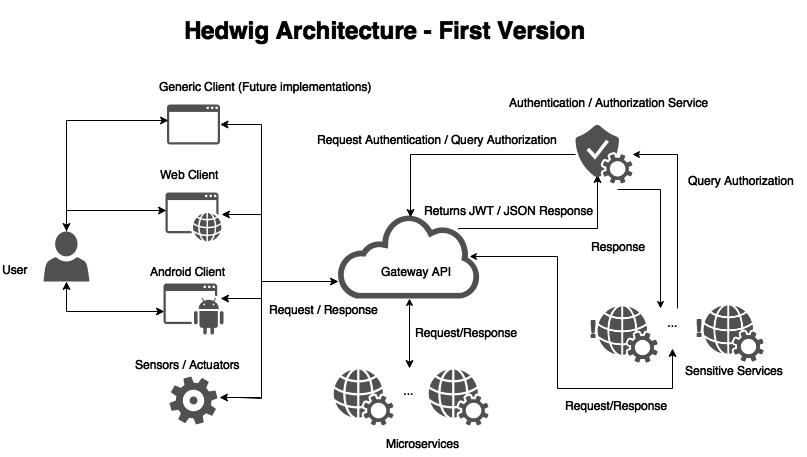
\includegraphics[width=0.8\textwidth]{arquiteturaV1}
\label{fig:arquiteturaV1}
\end{figure}

É possível observar que alguns microsserviços são classificados como sensitivos, os quais dependem de nova consulta ao serviço de autenticação e  autorização, para garantir a segurança. Esses serviços são todos aqueles responsáveis por tomar uma ação em relação à casa que envolva riscos. Os microsserviços não sensitivos utilizam a autenticação já realizada pelo gateway, na chegada do request.

Quando uma requisição chega à nuvem, ela deve ser autenticada, e caso passe nos critérios de autenticação e autorização, é retornado um JWT (JSON Web Token), necessário para os passos seguintes. O token JWT é discutido aqui, na seção MARCAR SEÇÃO AQUI.

De extrema importância, e não cobertos pela arquitetura anterior, são os requisitos de disponibilidade do projeto. Se o gateway estiver inacessível em determinado momento, a casa não terá mais nenhuma forma de comunicação com os meios externos, mesmo para os serviços mais básicos. Para resolver este problema, foi proposta uma segunda versão, conforme ilustra a imagem seguinte.

\begin{figure}[H]
	\centering
	\caption{Segunda versão da arquitetura do projeto Hedwig}
  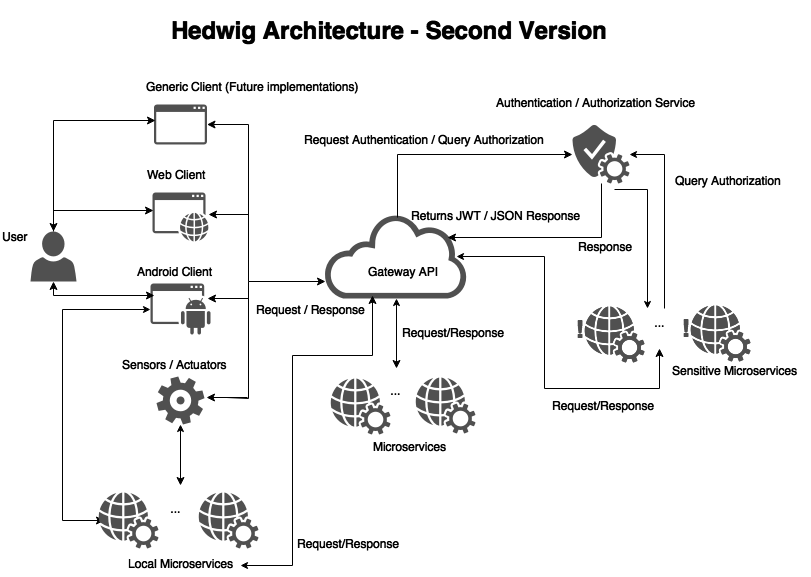
\includegraphics[width=0.8\textwidth]{arquiteturaV2}
\label{fig:arquiteturaV2}
\end{figure}

Nesta versão, serviços essenciais seriam duplicados dentro da casa, e no caso de haver qualquer forma de impedimento na comunicação com a nuvem, esses serviços seriam responsáveis por controlar diretamente os atuadores desejados. Entretanto, cria-se mais uma complexidade, ao manter serviços duplicados na casa, e no caso destes serviços não estarem online no momento necessário, também não seriam alcançados requisitos mais fortes de disponibilidade. Contudo, é uma versão que chega mais próximo de obedecer às necessidades do projeto.

Essa arquitetura provê módulos sem inteligência, e todo o controle é feito pelo serviço correspondente. Ao mesmo tempo que essa escolha tem benefícios, como a escalabilidade, a manutenção (já que é muito mais simples atualizar o software de um ponto único, sempre que necessário), para correções ou possíveis aumentos de funcionalidade. Porém, não ficaríamos livres, mais uma vez, do ponto único de falha. Também, alguns módulos ficariam em lugares de difícil acesso, ou mesmo fora da casa, onde a comunicação poderia ser perdida, ou ser intermitente. Assim, em caso de falha de comunicação, um atuador não receberia os sinais necessários do serviço, acarretando em sérios problemas de segurança. No caso de uma garagem, por exemplo, o portão permaneceria aberto indeterminadamente, ou poderia não ser aberto o morador chegasse em csa.

Assim, começamos o desenvolvimento de um modelo arquitetural modularizado, onde cada módulo teria inteligência para realizar as tarefas necessárias e, ao mesmo tempo, podendo enviar dados à nuvem, e ser avisado quando deve realizar uma tarefa. Com isso, em um aspecto também comercial, módulos inteiros poderiam ser vendidos, substituídos e aumentados.

A arquitetura escolhida, também faz uso de microsserviços, no lado da nuvem, e no lado da casa os componentes de hardware passam a ser agrupados em módulos independentes, com responsabilidades bem estabelecidas, inteligência para fazer todas as atividades necessárias, e com comunicação a um servidor local, que realizará, por último, a comunicação direta com os serviços não locais. Esse servidor se comunicaria com módulos por meio de mensagens, enviadas em tópicos, as quais seriam interpretadas e enviadas aos servidores remotos. Se a casa perder comunicação com a nuvem, o servidor local armazenará as mensagens, que serão enviadas posteriormente. Essas mensagens, no caso, seriam de dados, advindas de sensores em módulos. Como não há urgência para o processamento de tais dados, os quais serão utilizados para análise de comportamento e machine learning, não há prejuízo com o eventual envio tardio.

Quando a comunicação entre o servidor local e a nuvem for perdida, os aplicativos web ou mobile, poderão se comunicar diretamente com o servidor local da casa, para acessar uma quantidade mais restrita e essencial de ações (como liberação de acesso, por exemplo). Além disso, no caso de perda de comunicação com o servidor local também, os aplicativos poderão se comunicar diretamente com os módulos para terem acesso aos serviços de extrema importância.

Por ser escolhida, essa arquitetura será extensivamente detalhada e discutida aqui, com seus benefícios e limitações.

\section{Módulos}
Para a criação dos módulos de hardware, foram escolhidos componentes de IoT comerciais, que possuem preços acessíveis, ampla documentação disponível e uma comunidade de desenvolvedores crescente.

A interconexão dos componentes, bem como a comunicação com o mundo externo pela internet será intermediada por um servidor local, que rodará na plataforma Raspberry Pi, rodando um sistema operacional Linux (Raspbian), baseado em Debian, e que dispõe da interface de hardware necessária para conexão com a rede.

Os sensores e atuadores devem ser conectados fisicamente com um módulo controlador, de modo que, para contornarmos essa limitação, utilizaremos módulos ESP8266 para transmissão sem fio por meio do WiFi. Esses módulos serão responsáveis pela transmissão das informações recebidas para o servidor local. Toda a arquitetura para essa transmissão será detalhada mais à frente. Os outros módulos a serem utilizados, como sensores DHT11, LM555, etc,  podem ser vistos no anexo, em uma lista completa. % TODO precisa colocar essa lista no anexo

Em geral, esses módulos consistem do microcontrolador, relés, sensores e fontes/conversores de tensão a depender do módulo, além de um circuito para manutenção corretiva baseado no astável 555, conectados à rede WiFi e/ou trabalhando como pontos de acesso. Para casos de falha de conexão, há um algoritmo de novas tentativas com tempos progressivamente maiores conforme as falhas ocorrerem, que busca deixar o módulo disponível para outras funções enquanto o serviço não está disponível. Para evitar o travamento, um sinal de “keep alive” é monitorado, e um circuito anti travamento deve ativar um “hard reset” (reset por hardware), ou então uma rotina de “soft reset” deve ser acionada. No entanto, observe que a segunda alternativa é a mais fácil de implementar, mas a menos robusta, já que ainda pode não funcionar em casos de loop infinito.

\subsection{Módulos Base}
\subsubsection{ESP8266}
O ESP8266 é um microprocessador com baixo consumo e conexão WiFi 802.11 integrada \cite{espressif}. Pode ser programado usando a Arduino IDE, já muito utilizada \cite{thomsen}. Opera com uma tensão de 3.3 V, suporta WPA e possui modo de interrupção somente por software. É amplamente usado como shield para conexão WiFi de placas de desenvolvimento da plataforma Arduino; contudo, no projeto Hedwig, o utilizaremos em modo StandAlone como principal processador e responsável pela conexão dos diferentes módulos de automação. Suas duas principais plataformas de desenvolvimento são Wemos\footnote{Plataforma Wemos: https://www.wemos.cc/} e NodeMCU\footnote{Plataforma NodeMCU: http://nodemcu.com/}. O projeto utilizará o Wemos D1 Mini, versão compacta da Wemos D1 R2.

Possui um modo de operação de baixa potência (sleep mode), em que o nível de funcionalidades fica limitado, contudo o consumo de bateria fica muito menor. Podemos usar 7 portas de E/S digitais e uma porta de entrada analógica. Duas portas são inutilizáveis, pois são usadas para programação e outras tarefas do sistema integrado do ESP8266. Uma alternativa para extensão de portas é utilizar, por exemplo, três níveis de sinal análogico para detectar três tipos de acionamento (através de um circuito dedicado, com priorização de entrada), interface I2C (como o usado para o display) e uso de Radio Frequência, através de um par receptor-transmissor integrado no módulo, controles, atuadores e sensores sem fio.

% TODO tirar esse paragrafo abaixo daqui e coloca-lo em uma secao sobre o modulo de acesso a casa
Dentre os materiais adquiridos, destacam-se como exemplos o controle RF  e sensor de abertura de portão sem fio - observe que a fechadura eletrônica já existe na residência teste, logo é utilizada nesse projeto, contudo não está na lista de materiais para aquisição.

\subsubsection{Multiplexação no tempo}
Para tratar indisponibilidade dos módulos devido a tentativas de reconexão e conexão e requisições não gerenciadas e aumentar a disponibilidade, além do circuito antitravamento e hard reset, as diversas rotinas (desde configuração inicial, reconfigurações, coletas de dados, atuar por meio de relés, até conexão, desconexão, reconexão e envio de dados) foram multiplexadas no tempo da seguinte forma:

\begin{figure}[H]
	\centering
	\caption{Rotina de multiplexação de procedimentos no tempo}
  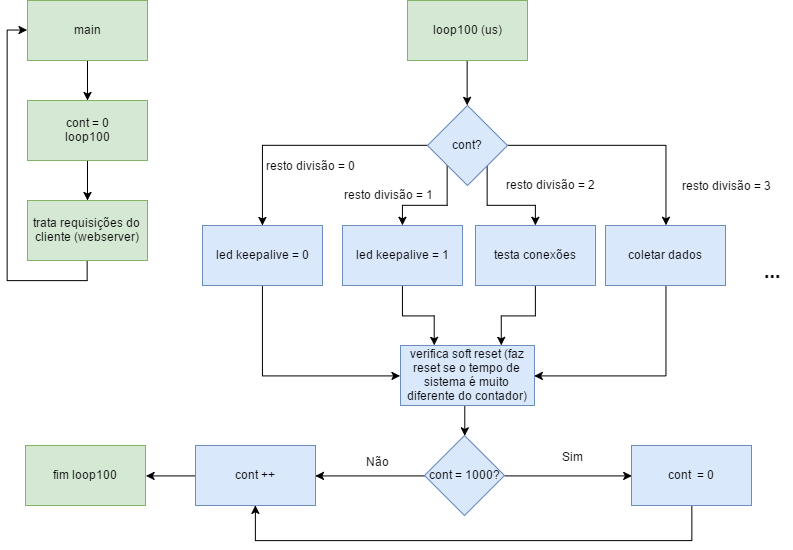
\includegraphics[width=0.8\textwidth]{rotinaMultiplexacao}
\label{fig:rotinaMultiplexacao}
\end{figure}

\subsubsection{Tratamento de indisponibilidade}
Nos casos de indisponibilidade de internet, servidor ou rede local, o seguinte procedimento foi adotado: (observe que a indisponibilidade do próprio módulo é tratada pelo circuito antitravamento).

\begin{figure}[H]
	\centering
	\caption{Tratamento de indisponibilidade de recursos}
  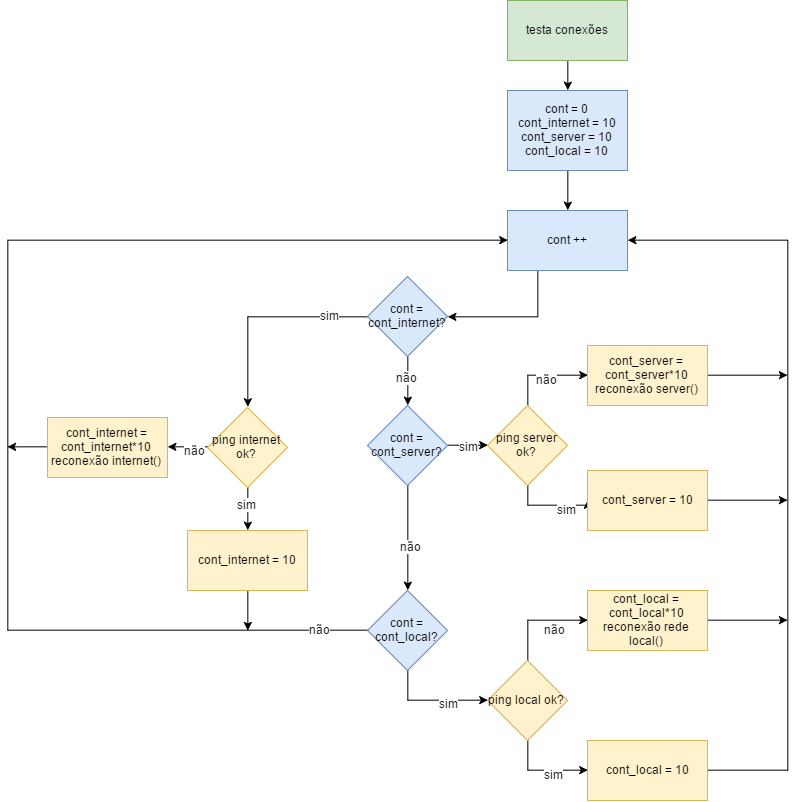
\includegraphics[width=0.8\textwidth]{tratamentoIndisponibilidade}
\label{fig:tratamentoIndisponibilidade}
\end{figure}

Com esse procedimento, as tentativas de reconexão à internet, servidor e rede local estão segregadas e com tentativas realizadas em intervalos de tempo sucessivamente maiores. Desta forma, conseguimos gerenciar esses procedimentos, já que o nível de processamento é baixo.

\subsubsection{DoS Local (Evil Twin)}
No caso de ataque de Evil Twin, no qual uma rede mal intencionada, usualmente aberta, usa o mesmo ssid da rede original, com o objetivo de obter a senha, o sistema pode ficar indisponível até ao nível local. Módulos podem se conectar à rede mal intencionada e ficarem somente com as funcionalidades offline (como acionamento de lâmpada por botão física acoplado ao módulo). Outro problema é a queda da rede por interferência de radio frequência ou outro mecanismo utilizado pelo usuário mal intencionado para que os clientes se desconectem, tentem reconexão e forneçam a senha da rede.

Para mitigar esses riscos, os módulos executam o seguinte procedimento:
\begin{figure}[H]
	\centering
	\caption{Tratamento de ataque de DoS Local}
  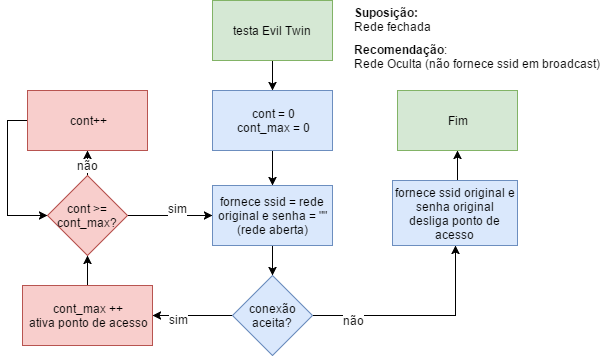
\includegraphics[width=0.8\textwidth]{tratamentoDoS}
\label{fig:tratamentoDoS}
\end{figure}

\subsubsection{Diagrama}
Segue diagrama do circuito impresso (PCB) feito em conjunto com o Projeto Katz-House\footnote{Katz-House, Fabio Hayashi. Projeto Pessoal, 2017.}. Funcionalidade, componentes e arquitetura foram responsabilidade do Projeto Hedwig, enquanto a disposição física, se atentando para problemas de interferência e mantendo um módulo menor possível foi responsabilidade do Projeto Katz-House.

\begin{figure}[H]
	\centering
	\caption{Diagrama PCB do Módulo Base}
  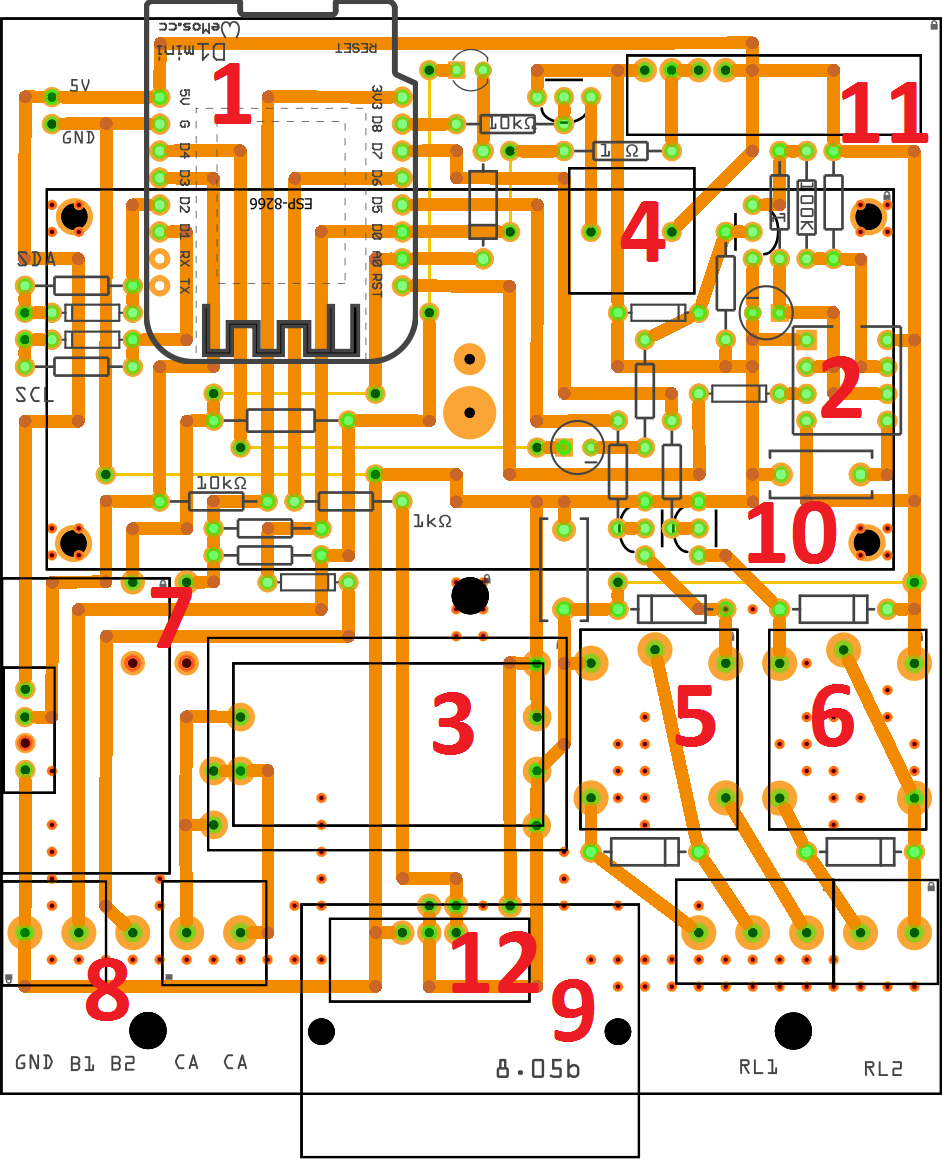
\includegraphics[width=0.8\textwidth]{diagramaModuloBase}
\label{fig:diagramaModuloBase}
\end{figure}

\begin{enumerate}
\item Wemos D1 mini
\item Astável 555
\item Fonte 5V 3W
\item Buzzer
\item Relé 1
\item Relé 2
\item Hard Reset
\item Botões
\item Presença
\item RF-RX
\item RF-TX
\end{enumerate}

\begin{figure}[H]
	\centering
	\caption{Diagrama PCB do Módulo Base}
  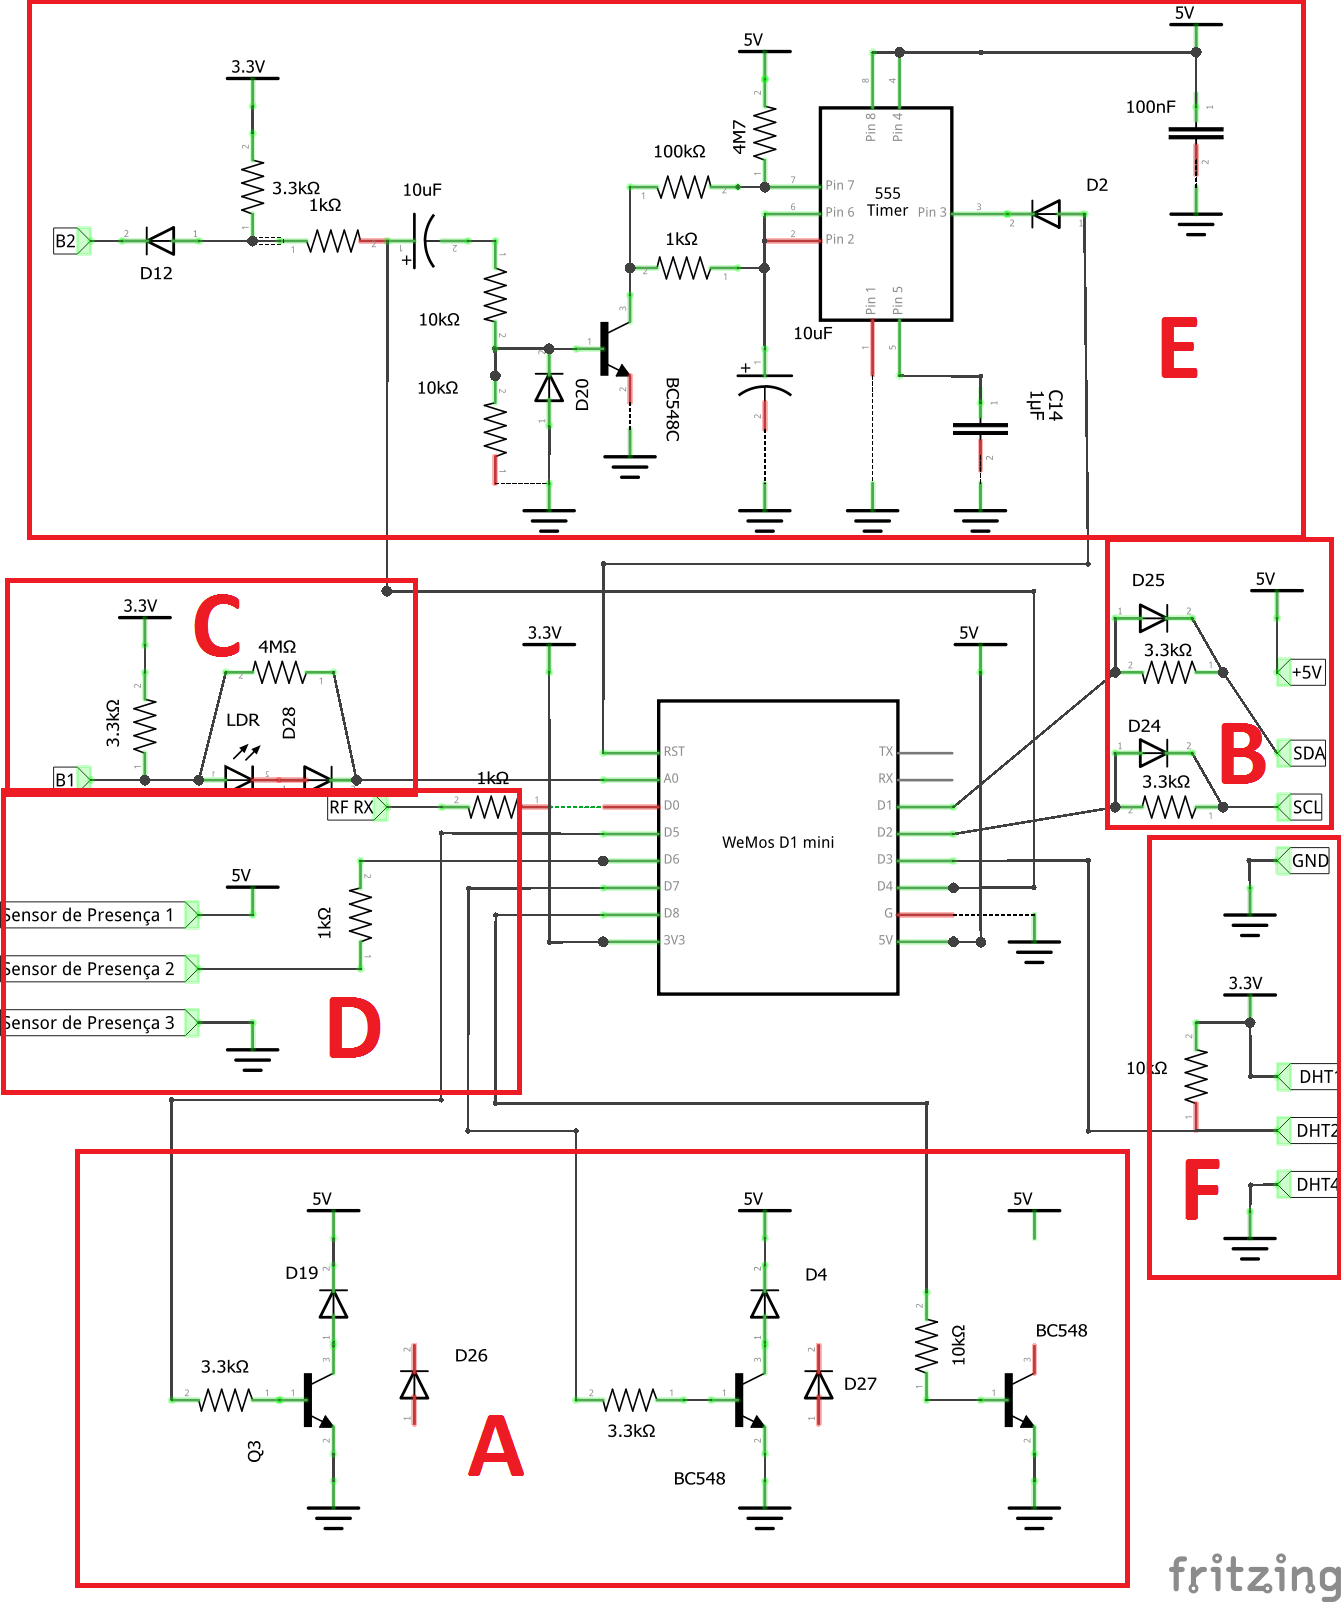
\includegraphics[width=0.8\textwidth]{esquematicoModuloBase}
\label{fig:esquematicoModuloBase}
\end{figure}

\begin{description}
\item [A - Saídas] Circuitos simples de transistor para acionamento de relés (para lâmpadas) e buzzer.
\item [Proteção 3V3 5V] Como o display trabalha com tensão de 5V, há proteções com diodos para não danificar as entradas digitais do Wemos D1 mini, que trabalha com tensão de 3V3.
\item [3 Entradas em A0] O circuito tem como entradas um botão (para acionamento do relé 1), o LDR (para chaveamento do backlight do display), e um outro botão para hard reset do dispositivo, todos numa entrada analógica, cujo mapeamento E/S é da seguinte forma:

\begin{figure}[H]
	\centering
	\caption{Entradas Em A0}
  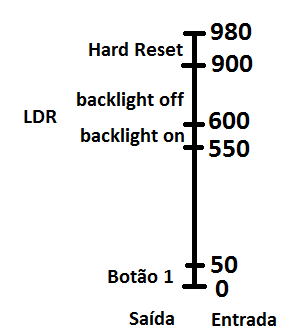
\includegraphics[width=0.4\textwidth]{entradasEmA0}
\label{fig:entradasEmA0}
\end{figure}

\item [Presença ou RF-TX] A entrada digital D6 é usada exclusivamente como entrada do sensor de presença PIR ou receptor RF.
\item [Astável 555 para Hard Reset e Botão] A porta D6 é usada como LED “keep alive” do módulo. Sua demora ao piscar indica que o módulo está travado ou demorando muito para processar algo (o que não deveria acontecer, uma vez que os procedimentos estão multiplexados no tempo, de acordo com seus tempos limite). Dessa forma, conectamos essa saída a um circuito antitravamento, que executa o reset caso nos casos mencionados, de travamento ou “timeout”.

O primeiro capacitor tem como objetivo desacoplamento DC, de forma que a entrada do circuito envolvendo o astável 555 seja somente AC. Assim, travamentos em 0 ou 1 indicam travamento.

Enquanto o led pisca em intervalos esperados (regularmente), o transistor conduz e mantém uma saída dente de serra muito próxima de 0. Quando o módulo trava, o transistor não conduz mais, e a saída passa a oscilar entre 1/3 e 2/3 da tensão total (observe que o carregamento é feito pelo resistor de 4M7, muito maior que o resistor de 100k, fazendo com que o tempo de carga seja muito maior que o tempo de descarga, uma vez que esses tempos são diretamente proporcionais à constante de tempo dos circuitos RC, que é dada pelo produto do R*C). Durante a descarga, o reset da placa é realizado. Observe que os tempos foram ajustados pelos valores dos componentes discretos, para que o tempo entre resets sucessivos seja menor que o tempo necessário para o módulo voltar a funcionar após um reset.

Segue abaixo uma ilustração sobre o funcionamento do circuito.

\begin{figure}[H]
	\centering
	\caption{Funcionamento do Circuito de Antitravamento}
  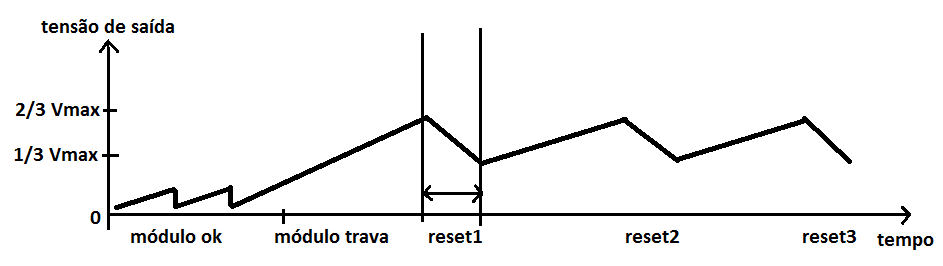
\includegraphics[width=0.8\textwidth]{circuitoAntiTravamento}
\label{fig:circuitoAntiTravamento}
\end{figure}

\item [DHT11] Entrada D3 é ligada a uma montagem básica para leitura de umidade e temperatura através do periférico DHT11.

\end{description}

\subsubsection{Montagem}

\subsection{Módulo de Interface com Sistema de Alarmes}
\subsubsection{Especificação}
\subsubsection{Montagem}

\subsection{Módulo de Acesso}
\subsubsection{Especificação}
\subsubsection{Montagem}

\subsection{Módulo de Quarto}
\subsubsection{Especificação}
\subsubsection{Montagem}

\subsection{Módulo de Aquário}
\subsubsection{Especificação}
\subsubsection{Montagem}

\subsection{Módulo de Cozinha}
\subsubsection{Especificação}
\subsubsection{Montagem}

\section{Controlador Local}
Para a intercomunicação entre os módulos e a nuvem, há a presença do servidor local Morpheus, responsável por introduzir mais uma camada de segurança, na troca de mensagens. Para isso, foi desenvolvido uma plataforma, com a utilização de mensageria, e a definição de um protocolo de comunicação entre os serviços de nuvem e os módulos. Assim, quando um usuário desejar realizar determinada operação por meio do cliente web, uma mensagem é enviada, a qual será interpretada pelo servidor local, e em seguida encaminhada para o destino, por meio do protocolo MQTT, com o broker Mosquitto.

\subsection{Raspberry Pi}
O Raspberry Pi é um computador integrado num único chip, do tamanho de um cartão de crédito. Foi desenvolvido com o objetivo de promover o ensino de computação básica, que possui funcionalidades tais como um computador desktop: navegação na internet, reprodução de video, processamento de texto, dentre outros. No projeto, será utilizado como servidor local (gerenciador de módulos local da casa), exatamente pelas funcionalidades compatíveis com a de um computador desktop.

A versão 3 possui uma CPU 1.2 Ghz 64-bit quad-core ARMv8, conexão 802.11n Wireless LAN, Bluetooth 4.1, suporte a Bluetooth Low Energy (BLE), 1GB RAM, 4 portas USB, 40 pinos GPIO, porta HDMI, porta Ethernet, interface para câmera, display e cartão SD. Para projetos que necessitem de baixo consumo energético, os modelos mais indicados são Pi Zero ou A+ \cite{raspPi}.

\section{Servidor na Nuvem}
Como foi escolhida uma arquitetura baseada microsserviços para construção do projeto, módulos diferentes podem ser escritos em linguagens de programação diferentes, o que promove uma maior flexibilidade não só durante o desenvolvimento dos módulos de mostrados nesse trabalho, mas também daqueles projetados futuramente como extensões do sistema Hedwig.

Para o desenvolvimento dos módulos definidos na especificação do projeto, utilizamos tecnologias atuais que são utilizadas em grandes empresas de tecnologia do mundo e possuem vasta documentação, referências e fontes de conhecimento como tutoriais e exemplos.
Para o desenvolvimento da parte de software, utilizaremos tecnologias atuais, que são também utilizadas nas maiores empresas de tecnologia do mundo. De acordo com o planejamento, utilizaremos uma arquitetura de microsserviços para construção do projeto. Com esta técnica, módulos diferentes poderiam ser escritos em, inclusive, linguagens de programação diferentes, o que promove uma maior flexibilidade durante o desenvolvimento.
Para o desenvolvimento da API, responsável pelos módulos sendo executados na nuvem e comunicação com banco de dados, utilizaremos Node.js (interpretador de código JavaScript do lado do servidor), com a utilização de alguns frameworks como é o caso do Express. O banco de dados com a qual ela se conecta é do tipo MongoDB (banco de dados orientado a documentos). Tais decisões foram baseadas no fato de bancos de dados em MongoDB serem altamente escaláveis e flexíveis, assim como Node.js, que, por sua arquitetura movida a eventos de E/S que não bloqueiam o servidor, provê ao mesmo uma altíssima escalabilidade, ao permitir milhares de conexões simultâneas, sem impacto na performance do servidor. Além disso, o fato de que os dados provindos do banco já estão organizados em objetos, e dessa forma, podem ser recebidos prontamente como objetos JavaScript no código em Node.Js geram facilidade e fluidez para o desenvolvimento do código.

\subsection{Arquitetura de Microsserviços}
\subsubsection{Características}
A arquitetura de microsserviços é um estilo que compreende a estruturação de uma aplicação em um conjunto de serviços com baixo grau de acoplamento que se comunicam por meio de protocolos de comunicação leves.

Para melhor compreender essa arquitetura, podemos compará-la à arquitetura monolítica. Uma aplicação monolítica está contida em uma única unidade, que geralmente é dividida em camadas de funcionalidade tecnológica como interface web, camada de negócios server-side e camada de persistência de dados. A escalabilidade desse modelo é dada por meio do aumento do número de servidores, máquinas virtuais ou contêineres juntamente a um load balancer - é a chamada escalabilidade horizontal. Uma alteração em uma pequena parte da aplicação significa que toda a aplicação deverá passar por um processo de build e deploy. Já a arquitetura de microsserviços divide as funcionalidades em serviços autônomos, muitas vezes usando as regras de negócios para realizar essa divisão. Cada serviço tem seu próprio ciclo de desenvolvimento e pode ser atualizado independentemente. A escalabilidade também é tratada serviço a serviço.

\begin{figure}[H]
	\centering
	\caption{Comparação entre uma aplicação monolítica (esquerda) e com microsserviços (direita)}
  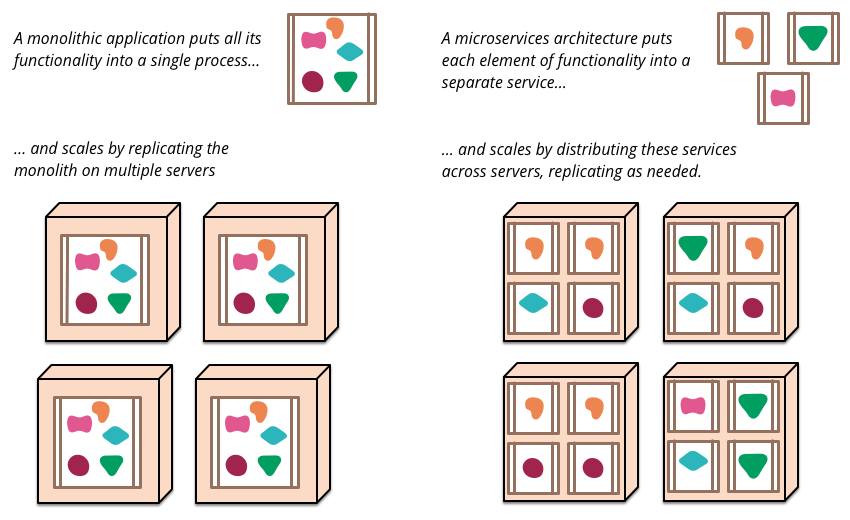
\includegraphics[width=0.8\textwidth]{estruturaMicrosservicos}
\label{fig:estruturaMicrosservicos}
\end{figure}

É difícil delimitar uma definição formal para arquitetura de microsserviços, pois não existe consenso a respeito de sua definição formal. Contudo, existe uma série de características que projetos usando essa arquitetura compartilham. Detalhamos a seguir alguns atributos e aspectos dos microsserviços. Nem todos os projetos possuem rigorosamente todas as características, mas a maioria deles possui um perfil similar ao descrito aqui.

\begin{itemize}
\item \textbf{Serviços são processos. }Pode-se fazer um mapeamento de um processo para um serviço, porém isso é apenas uma aproximação, podendo um serviço ser constituído por uma aplicação de múltiplos processos.
\item \textbf{Serviços comunicam-se por protocolos leves. }Geralmente, são usados protocolos como o HTTP.
\item \textbf{Serviços implementam capabilidades do negócio. }Isto é, a divisão de serviços é baseada nas regras de negócio e nas funcionalidades que o produto deverá suprir.
\item \textbf{Serviços são facilmente substituíveis.}
\item \textbf{Cada serviço tem um ciclo de vida independente. }Isso inclui o desenvolvimento e os processos de deploy. Um microsserviço pode ser implementado e atualizado independentemente dos outros.
\end{itemize}

As vantagens da arquitetura de microsserviços giram em torno da modularidade e autonomia dos serviços que é natural à sua estrutura. Com isso, pode-se ter uma heterogeneidade de tecnologias, isto é, cada serviço pode ser desenvolvido usando diferentes linguagens, frameworks e ferramentas de acordo com seus requisitos. A independência entre serviços também possibilita o deploy automatizado e o uso de práticas de integração contínua. Também há benefícios de aspecto gerencial: como cada serviço tem como escopo uma capabilidade do negócio que envolve interfaces de interação com usuário, código em várias camadas que implementa as funcionalidades necessárias e persistência em bancos de dados, é possível criar pequenas equipes multidisciplinares para cada microsserviço.

Building for failure % TODO

Existem trade-offs que devem ser considerados ao decidir pela arquitetura de microsserviços. A comunicação entre serviços por meio de uma rede possui maior latência e exige maior processamento do que mensagens trocadas a nível de processos. Por isso, é muito importante analisar as fronteiras dos serviços e a alocação de responsabilidades durante do projeto. A descentralização de dados entre microsserviços traz também a necessidade de métodos para manter a consistência das informações. Outro ponto crítico são sistemas com alta granularidade de microsserviços, causando overhead tanto de comunicação como de código além de uma fragmentação lógica que causa mais impactos negativos na complexidade e performance do que benefícios - tal caso de antipadrão foi chamado de nanosserviço \cite{rotem}.

% TODO melhorar paragrafo abaixo
Os microsserviços podem ser vistos como um estilo específico de arquitetura orientada a serviços (Service-oriented architecture - SOA), visto que existem várias características compartilhadas entre os dois. Contudo, o termo arquitetura orientada a serviços é muito amplo, e muitas de suas implementações podem não seguir certos pontos apresentados como aspectos dos microsserviços, como por exemplo, o uso de grande inteligência no mecanismo de comunicação de dados ao invés de delegar tal complexidade aos endpoints do serviço \cite{james}. Esse e outros problemas conhecidos das experiências passadas de sistemas estruturados em SOA fazem com que muitos encarem os microsserviços como uma modernização da arquitetura orientada a serviços.

Apesar do termo microsserviço ter surgido por volta de 2011 \cite{james}, as ideias por trás desse estilo arquitetural não são recentes. O aumento da discussão em torno dos microsserviços nos últimos anos pode ser creditada a avanços tecnológicos tais como a disseminação dos serviços de nuvem, o crescimento de ferramentas de automatização de deployment, a consolidação dos conceitos de DevOps, entre outros.

\subsubsection{Casos de uso} % TODO

\subsubsection{Microsserviços e Internet das Coisas} % TODO

\section{Cliente Web}
Para criar aplicações web que demonstrem as funcionalidades dos módulos de automação da casa, foi escolhida a biblioteca de JavaScript React, que permite o fácil desenvolvimento de aplicações single-page, renderizadas do lado do cliente, e que permitem a atualização dinâmica da página, de forma fluida, rápida, o que acaba enriquecendo a experiência do usuário na aplicação (UI e UX). Esse cliente irá se comunicar com a API, por meio do protocolo HTTP, e utilizando autenticação de usuário por meio  de tokens do tipo JSON Web Token. JSON Web Tokens são tokens gerados no cadastro ou login do usuário, e são enviados ao browser, onde são armazenados na Localstorage do mesmo.

A partir desse momento, todas as requisições ao back end conterão tal token no campo de Authentication do cabeçalho dos métodos HTTP (GET, PUT, POST, DELETE). Somente requisições contendo tal token, e cujo token seja válido, são aceitas.

Outro ponto interessante para a utilização da biblioteca React é que, com a biblioteca React Native - uma extensão da biblioteca React - é possível a geração de aplicativos nativos para iOS e Android, que podem vir a ser desenvolvidos no desenrolar do projeto. Isso diminui a necessidade de retrabalho e dispensa a necessidade de estudo aprofundado das linguagens e ambientes de desenvolvimento tradicionais de projeto de aplicativos nativos.

\section{App Backup}
\subsection{Interface}
\subsection{Setup}
\subsection{Abertura de porta do roteador}
\subsection{Configurações}
\subsection{Serviços essenciais}

\section{Comunicação}
Conforme explicado anteriormente, neste projeto utilizamos tanto protocolos de comunicação próprios quanto os elaborados comercialmente. A arquitetura desenvolvida aqui busca viabilizar a robustez do sistema, trabalhando em um nível local e outro nível remoto, onde o usuário terá o controle de sua casa por meio do Smartphone ou computador pessoal.

Teremos um serviço de nuvem (que será descrito na seção de software) que receberá as requisições do usuário, por meio de um cliente web ou nativo. Esse servidor processará as requisições, aplicando os filtros de segurança necessário, de modo a consultar a autenticidade do pedido, e se aquele usuário possui as permissões necessárias para o serviço que deseja operar. Os serviços da nuvem se comunicarão com o servidor local, da casa requisitada, o qual também aplicará os filtros de segurança necessários, e realizará a comunicação com os atuadores.

A infraestrutura de comunicação entre a nuvem e o servidor local, e o servidor local e os sensores e atuadores utilizará o protocolo de aplicação MQTT, referência em aplicações IoT no mundo. O protocolo MQTT é estabelecido em cima dos protocolos TCP/IP (nas camadas inferiores) e é orientado é orientado à sessão, diferentemente do protocolo HTTP, de mesma camada.

O protocolo MQTT é do tipo Pub/Sub (de publisher/subscriber) e é estritamente orientado à tópicos. Assim, um subscriber deve se inscrever a um tópico de seu interesse, e receberá todas as publicações que um publisher realizar. Os tópicos são organizados com estrutura semelhante a de um sistema de arquivos Unix, com níveis hierárquicos, separados por barras, de modo que o subscriber pode se inscrever para tópicos utilizando wildcards (* e +, os quais são válidos para mais de um nível e um único nível, respectivamente).

Para interconectar os tópicos, com publishers e subscribers, é necessário um agente que realiza a transmissão das mensagens, e que garante a segurança e confiabilidade. Esse agente é conhecido como Broker (em versões anteriores) ou Server (na versão atual, V3.1.1). O broker irá permitir ou negar a subscrição a determinado tópico, ou a publicação.

A segurança da troca de mensagens é realizada por meio do protocolo TLS (Transport Layer Security) que encripta os segmentos na camada de transporte. Toda a parte de segurança e criptografia será detalhada no momento oportuno, bem como a organização dos tópicos implementados.

Além disso, o protocolo MQTT oferece três tipos de QoS (Quality of Service), possibilitando: diminuir o overhead ao máximo, enviando a mensagem uma única vez, na configuração mais simples; garantir que a mensagem seja entregue no mínimo uma vez, na configuração de segundo nível; garantir que a mensagem seja entregue exatamente uma vez, no terceiro nível, o que aumenta o overhead, consequentemente.

As mensagens são transmitidas em texto puro, e é necessário estabelecer um protocolo para a sua utilização. Utilizaremos aqui o protocolo que define a configurações das mensagens, desenvolvido no projeto HomeSky.

O broker Mosquitto será utilizado, e foi escolhido por ser amplamente adotado em projetos de IoT, além de ser open source e com licença abrangente (MIT). Entretanto, há diversas possibilidades, como o HiveMQ, adotado no projeto HomeSky, e com grande uso em aplicações enterprise.

A arquitetura de comunicação é representada pelo diagrama abaixo, com um alto nível de abstração, cujos detalhes serão vistos no momento oportuno, com granularidade menor.

% TODO o diagrama ta diferente no arquivo da quarta entrega
% TODO update: Provavelmente esta certo agora, mas precisamos confirmar

\begin{figure}[H]
	\centering
	\caption{}
  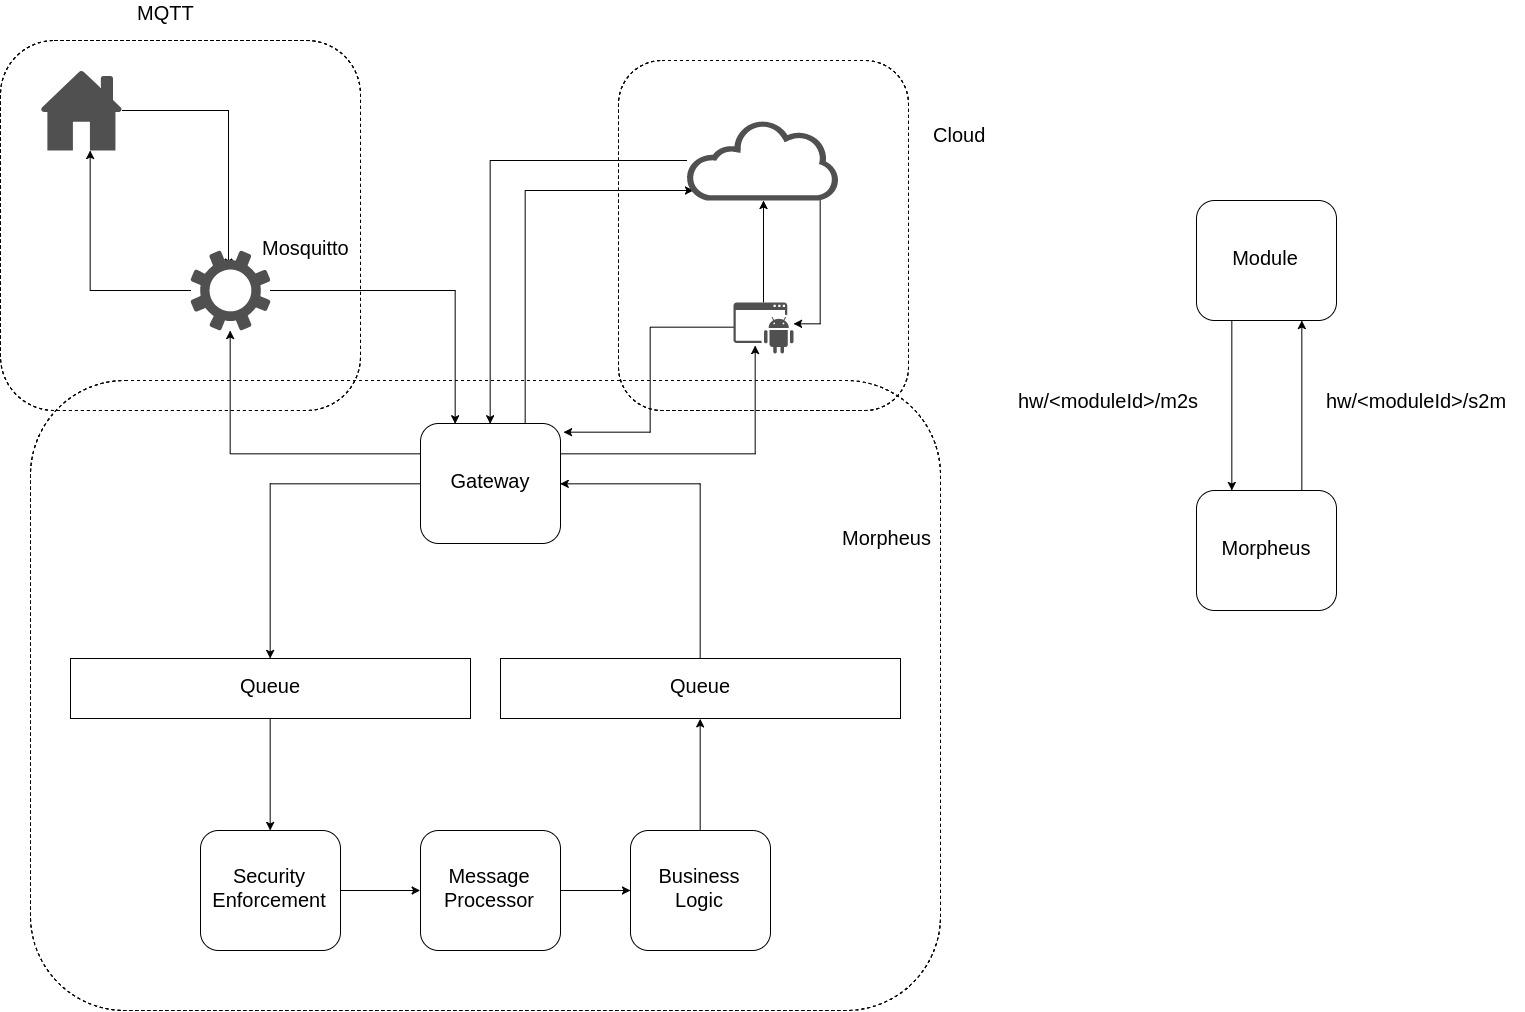
\includegraphics[width=0.8\textwidth]{diagramaComunicacao}
\label{fig:diagramaComunicacao}
\end{figure}

\subsection{Entre módulos e controlador local}
\subsection{Entre controlador local e nuvem}
\subsection{Entre cliente web e nuvem}
\subsection{Entre app backup e módulos}
